\section{Auswertung}
\label{sec:Auswertung}

Im folgenden werden die grundlegenden Eigenschaften des Ultraschalles, die in dem Versuch untersucht wurden, ausgewertet. \newline
Zunächst wurden die verwendeten Acrylkörper, also die Zylinder und Platten, abgemessen. Die gemessenen Werte sind in den beiden Tabellen 
\ref{tab:koerper1} und \ref{tab:koerper2} zu finden.

\begin{table}
  \centering
  \caption{Messwerte der Acrylzylinder.}
  \label{tab:koerper1}
  \begin{tabular}{c c c}
    \toprule
    Zylinder $Z_i$ & Durchmesser / $\si{\milli\meter}$ &  Länge $\si{\milli\meter}$\\
    \midrule
    $Z_4$ & 40 & 120,5 \\
    $Z_3$ & 40 & 80,5 \\
    $Z_2$ & 40,5 & 61,5 \\
    $Z_1$ & 40 & 40,4 \\
    \bottomrule
  \end{tabular}
\end{table}

\begin{table}
  \centering
  \caption{Messwerte der Acrylplattten.}
  \label{tab:koerper2}
  \begin{tabular}{c c}
    \toprule
    Platte $P_i$ & Dicke / $\si{\milli\meter}$ \\
    \midrule
    $P_1$ & 10 \\
    $P_2$ & 6 \\
    \bottomrule
  \end{tabular}
\end{table}

Die in \autoref{fig:reflexe} aufgenommene Grafik zeigt die vier Reflexe. Die Amplituden und Laufzeiten, die sich aus diesen Reflexen ergeben sind in \autoref{tab:refl}
eingetragen.

\begin{figure}[H]
  \centering
  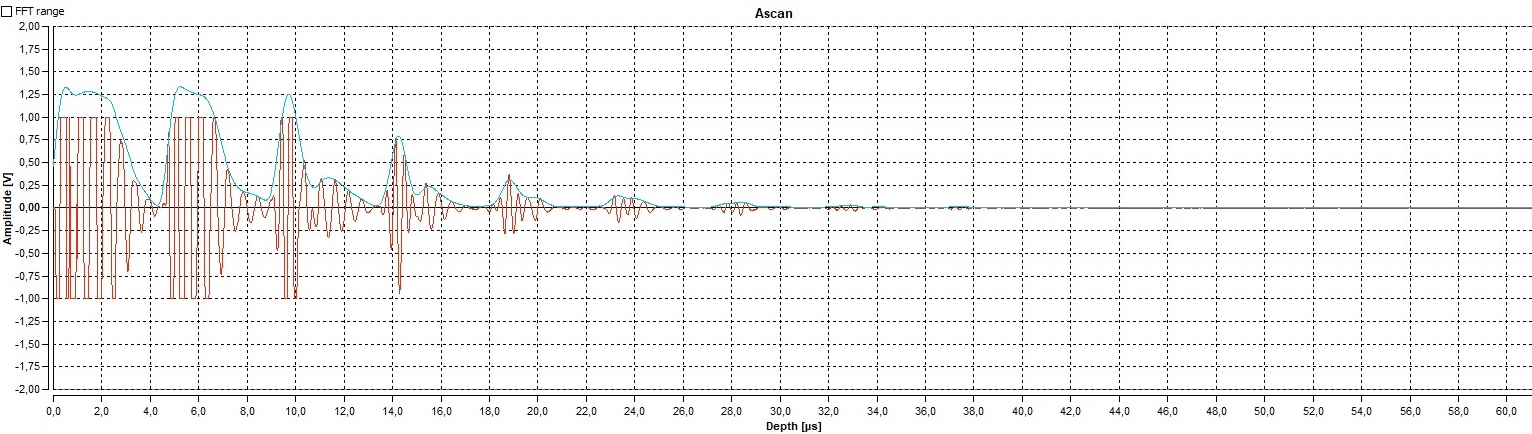
\includegraphics[width = \textwidth]{data/Geräteeinstellungen/reflexe.png}
  \caption{Aufgenommene Grafik zu den vier Reflexen.}
  \label{fig:reflexe}
\end{figure}

\begin{table}
  \centering
  \caption{Auswertung der aufgenommenen Grafik zu den vier Reflexen.}
  \label{tab:refl}
  \begin{tabular}{c c c}
    \toprule
    Reflex $R_i$ & Laufzeit / $\si{\micro\second}$ & Amplitude / $\si{\volt}$ \\
    \midrule
    $R_1$ & 4 & 1,3 \\
    $R_2$ & 4,9 & 1,3 \\
    $R_3$ & 4,8 & 1,25 \\
    $R_4$ & 3,2 & 0,8 \\
    \bottomrule
  \end{tabular}
\end{table}